\section{Versuch}
\subsection{Versuchsaufbau}
Die benutzten Werkzeuge sind der PtIr-Draht, ein Seitenschneider, eine Zange, eine Pinzette, die Proben HOPG und Gold, sowie das Rastertunnelmikroskop mit einer Abdichtung in der eine Lupe mit zehnfacher Verstärkung verbaut ist.

\noindent Die in Kapitel \ref{kap2} beschriebene Schwierigkeit der Vibrationen wird durch einen Schwingungsdämpfenden Tisch der zusätzlich auf vier dämpfenden Füßen steht, gelöst. Der Tisch ist aus Granit um eine möglichst schwere Grundfläche zu gewährleisten. Die Füße sind aus Gummi, um ein Verrutschen der Vorrichtung zu verhindern und sind intern mit Federn ausgestattet um die letzten Schwingungen zu dämpfen. Auf dem Tisch ist die Messvorrichtung installiert.

\noindent Ein Aufbau ist in Abbildung \ref{fig:Aufbau1} \cite{handbuch} dargestellt. 

\begin{figure}
	\centering
		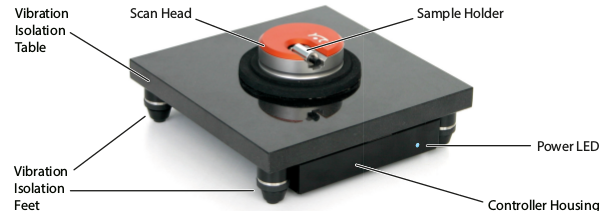
\includegraphics[width=0.5\textwidth]{Aufbau1.png}
	\caption{Rastertunnelmikroskop}
	\label{fig:Aufbau1}
\end{figure}

\noindent Ein genauerer Einblick in die Messvorrichtung wird in Abbildung \ref{fig:Aufbau2} gegeben.

\begin{figure}
	\centering
		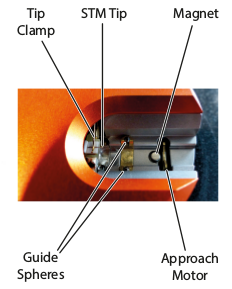
\includegraphics[width=0.5\textwidth]{Aufbau2.png}
	\caption{Messvorrichtung}
	\label{fig:Aufbau2}
\end{figure}

\noindent Durch den Magnet wird die Probenhalterung, die an ihrer Spitze selbst magnetisiert ist um die Probe, die auf einer kreisförmigen Metallscheibe liegt, an ihrem Ort fixiert. Die Spitze wird unter einen Bügel in eine dafür vorgesehene Furche gelegt und dort festgehalten. Die Probe kann auf metall Kugeln durch den Motor an den gewünschten Ort verschoben werden.

\subsection{Versuchsdurchführung}
Zunächst wurden die Werkzeuge mit 2-Propanol gereinigt. Mit der Zange wurde ein Stück des Drahts festgehalten und mit dem Seitenschneider wurde dann (nahezu parallel zur Zange gehalten) eine Spitze aus dem Draht gerissen. Zuletzt wurde die Spitze auf die richtige Größe geschnitten und mit der Pinzette unter den Bügel gelegt.

\noindent Daraufhin wurde eine Probe in die Messvorrichtung gelegt. Sie kann über die thermisch isolierte Halterung mit der Hand angefasst transportiert werden. Die Abdichtung wurde darauf gestellt.

\noindent Der Rest der Durchführung geschah mit dem Programm ''Nanosurf NaioSTM''.

\noindent Als Erstes wurde über den ''more''-Button das Menü für die SPM-Parameter geöffnet und unter ''Imaging'' -> ''Imaging Modes'' -> ''Scan Mode'', ''Scan Fw. \& Bw.'' ausgewählt.

\noindent Mit ''Advance'' bzw. ''Approach'' konnte die Spitze an die Probe gefahren werden. Nachdem die richtigen Parameter unter ''Parameters'' eingestellt wurden, musste noch eine Spannung (\(50\)mV) zwischen Spitze und Probe angelegt werden. Dies geschah durch die Einstellung unter ''Mode Properties''.